\documentclass{article}
\usepackage[utf8]{inputenc}
\usepackage{natbib}
\usepackage{epsf}
\usepackage{graphicx}
\setcounter{secnumdepth}{3}
%\usepackage{rotating}
\usepackage{multirow}
\usepackage[toc,page]{appendix}
\usepackage{placeins}
\usepackage{epsfig}

\usepackage{times}
\usepackage[utf8]{inputenc}
\usepackage{amsmath}
\usepackage{amssymb}
\usepackage{epsf}
\usepackage{graphicx}
\setcounter{secnumdepth}{3}
%\usepackage{rotating}
\usepackage{multirow}
\usepackage[toc,page]{appendix}
\usepackage{placeins}
\usepackage{epsfig}
%\usepackage{subfigure}
\usepackage{makeidx}
\usepackage{url}


%\usepackage{subfigure}
\usepackage{makeidx}
\usepackage{url}
%\usepackage[margin=1cm,labelfont=bf,font={small}]{caption}
\usepackage{fancyhdr}
\usepackage[headsep=0.5cm,headheight=3cm]{geometry}
\usepackage{sectsty}
\usepackage{longtable}
\usepackage{caption}
\usepackage{subcaption}
\usepackage{enumitem}
\usepackage{titlesec}
\usepackage{hyperref}
\usepackage{lipsum}
\usepackage{adjustbox}
\usepackage{threeparttable}
\usepackage{pdflscape}

\title{X-ray timing and spectral analysis of reverberating active galactic nuclei}
\author{Stephen Hancock}
\date{March 2022}

\begin{document}

\maketitle

\addcontentsline{toc}{section}{List of Tables}
\thispagestyle{empty}
\listoftables

\addcontentsline{toc}{section}{List of Figures}
\thispagestyle{empty}
\listoffigures


\begin{landscape}
\begin{longtable}{ccccccccc}
\caption[All AGN groups Relxill spectral fits]{The best spectral fits for AGN groups computed to 90\% confidence, outlining the model flux (2-10 keV erg cm$^{-2}$ s$^{-1}$), photon index $\Gamma$, ionisation $\log\xi$ (erg cm s$^{-1}$), iron abundance $A_\text{Fe}$ (solar), reflection fraction $RF$, disk inclination $i$ (deg) and the covering fraction (if applied).} \\ \hline
\label{spec_results}
\multicolumn{1}{c}{Source} & \multicolumn{1}{c}{Group} & \multicolumn{1}{c}{$F_{2-10}$ kev} & \multicolumn{1}{c}{$\Gamma_\texttt{Relxill}$} & \multicolumn{1}{c}{$\log \xi$} & \multicolumn{1}{c}{$AF_e$} & \multicolumn{1}{c}{RF} & \multicolumn{1}{c}{$\textit{i}$} & \multicolumn{1}{c}{Cvr Frac} \\ \hline 
\endfirsthead

\multicolumn{9}{c}%
{{\tablename\ \thetable{} -- continued from previous page}} \\
\hline \multicolumn{1}{c}{Source} & \multicolumn{1}{c}{Group} & \multicolumn{1}{c}{$F_{2-10}$ kev} & \multicolumn{1}{c}{$\Gamma_\texttt{Relxill}$} & \multicolumn{1}{c}{$\log \xi$} & \multicolumn{1}{c}{$AF_e$} & \multicolumn{1}{c}{RF} & \multicolumn{1}{c}{$\textit{i}$} & \multicolumn{1}{c}{Cvr Frac} \\ \hline 
\endhead

\hline \multicolumn{9}{r}{{Continued on next page}} \\ 
\endfoot

\hline \hline
\endlastfoot

\hline
1H0707-495 & Combined & 9.27 $\times 10^{-13}$ & $3.38^{+0.02}_{-0.02}$ &  $2.43^{+0.03}_{-0.03}$ & $0.50^{+0.03}_{-0.00}$ & $2.14^{+0.15}_{-0.15}$ & $74.90^{+0.99}_{-1.52}$ & $0.65^{+0.02}_{-0.02}$\\
& hi & 1.04 $\times 10^{-12}$ & $3.40^{+0.00}_{-0.02}$ & $2.44^{+0.08}_{-0.03}$ & $0.50^{+0.04}_{-0.00}$ & $2.13^{+0.15}_{-0.14}$ & $76.68^{+0.69}_{-1.04}$ & $0.63^{+0.01}_{-0.01}$\\
& hi cts s$^{-1}$ & 1.02 $\times 10^{-12}$ & $3.40^{+0.00}_{-0.02}$ & $2.56^{+0.08}_{-0.08}$ & $0.50^{+0.10}_{-0.00}$ & $2.16^{+0.15}_{-0.14}$ & $80.00^{+0.00}_{-0.70}$ & $0.65^{+0.02}_{-0.02}$\\
& med & 5.58 $\times 10^{-13}$ & $2.80^{+0.14}_{-0.34}$  & $3.58^{+0.16}_{-0.32}$ & $10.00^{+0.00}_{-1.64}$ & $4.98^{+3.30}_{-2.70}$ & $76.10^{+1.09}_{-0.57}$ & $0.83^{+0.03}_{-0.16}$\\
& lo & 2.99 $\times 10^{-13}$ & $2.73^{+0.12}_{-0.16}$ & $2.85^{+0.18}_{-0.15}$ & $9.59^{+0.41}_{-0.49}$ & $9.95^{+0.05}_{-4.98}$ & $80.00^{+0.00}_{-2.99}$ & $0.95^{+0.00}_{-0.01}$\\ 
& lo cts s$^{-1}$ & 3.28 $\times 10^{-13}$ & $2.95^{+0.35}_{-0.29}$ & $0.87^{+0.57}_{-0.29}$ & $10.00^{+0.00}_{-6.01}$ & $7.31^{+2.69}_{-3.85}$ & $80.00^{+0.00}_{-3.18}$ & $0.63^{+0.16}_{-0.00}$\\ \hline

Ark 564 & Combined & 1.87 $\times 10^{-11}$ & $2.36^{+0.06}_{-0.03}$ & $1.30^{+0.40}_{-0.25}$ & $4.99^{+5.01}_{-2.02}$ & $0.64^{+0.44}_{-0.26}$ & $75.60^{+1.81}_{-1.76}$ & -- \\ 
& hi & 1.92 $\times 10^{-11}$ & $2.31^{+0.01}_{-0.04}$  & $3.65^{+0.12}_{-0.29}$ & $10.00^{+0.00}_{-2.61}$ & $0.05^{+0.24}_{-0.01}$ & $22.10^{+22.40}_{-21.40}$ & -- \\
& lo & 1.09$\times 10^{-11}$ & $2.25^{+0.09}_{-0.09}$  & $3.48^{+0.20}_{-1.37}$ & $0.50^{+0.41}_{-0.00}$ & $8.69^{+1.31}_{-7.09}$ & $80.00^{+0.00}_{-12.40}$ & -- \\ \hline 

IRAS 13224-3809 & Combined & 6.36 $\times 10^{-13}$ & $3.25^{+0.04}_{-0.02}$ &  $2.13^{+0.06}_{-0.06}$ & $0.50^{+0.11}_{-0.00}$ & $3.20^{+0.36}_{-0.37}$ & $77.51^{+1.39}_{-1.18}$ & $0.60^{+0.02}_{-0.02}$ \\ 
& hi & 1.23 $\times 10^{-12}$ &  $3.17^{+0.09}_{-0.08}$ &  $1.41^{+0.39}_{-0.01}$ & $2.79^{+1.40}_{-2.02}$ & $2.16^{+0.41}_{-0.24}$ & $77.82^{+2.18}_{-2.19}$ & $0.29^{+0.15}_{-0.09}$ \\ 
& hi cts s$^{-1}$ & 6.45 $\times 10^{-13}$ &  $3.13^{+0.09}_{-0.08}$ &  $0.92^{+0.17}_{-0.04}$ & $0.50^{+0.24}_{-0.00}$ & $4.02^{+0.99}_{-1.02}$ & $77.29^{+1.48}_{-1.64}$ & $0.22^{+0.07}_{-0.05}$ \\ 
& med & 5.30 $\times 10^{-13}$ &  $3.27^{+0.00}_{-0.00}$ & $2.12^{+0.01}_{-0.01}$ & $0.86^{+0.01}_{-0.01}$ & $3.09^{+0.22}_{-0.21}$ & $72.30^{+0.35}_{-0.40}$ & $0.63^{+0.00}_{-0.00}$ \\ 
& lo & 2.57 $\times 10^{-13}$ &  $3.14^{+0.06}_{-0.21}$ & $1.87^{+0.16}_{-0.13}$ & $0.50^{+0.71}_{-0.00}$ & $9.24^{+0.76}_{-4.06}$ & $65.46^{+3.35}_{-2.32}$ & $0.74^{+0.03}_{-0.11}$ \\
& lo cts s$^{-1}$ & 4.21 $\times 10^{-13}$ &  $3.20^{+0.00}_{-0.00}$ &  $1.83^{+0.06}_{-0.08}$ & $0.50^{+0.01}_{-0.00}$ & $2.92^{+0.37}_{-0.38}$ & $74.68^{+1.09}_{-1.41}$ & $0.64^{+0.00}_{-0.00}$ \\ \hline 


MCG-6-30-15 & Combined & 4.12 $\times 10^{-11}$  & $2.00^{+0.02}_{-0.12}$ & $3.01^{+0.02}_{-0.12}$ & $10.00^{+0.00}_{-0.36}$ & $10.00^{+0.00}_{-4.99}$ & $32.16^{+2.79}_{-2.42}$ & --\\ 
& hi & 4.64 $\times 10^{-13}$ & $2.00^{+0.13}_{-0.10}$ & $3.01^{+0.03}_{-0.11}$ & $10.00^{+0.00}_{-0.52}$ & $10.00^{+0.00}_{-0.54}$ & $32.06^{+2.47}_{-2.21}$ & --\\
& lo & 3.24 $\times 10^{-11}$ & $1.78^{+0.06}_{-0.08}$ & $2.82^{+0.18}_{-0.29}$ & $10.00^{+0.00}_{-5.54}$ & $0.77^{+0.52}_{-0.31}$ & $41.98^{+5.97}_{-5.66}$ & --\\  \hline 

Mrk 335 & Combined  & 9.58 $\times 10^{-12}$ & $2.82^{+0.28}_{-0.20}$ & $0.82^{+0.25}_{-0.39}$ & $0.78^{+1.47}_{-0.23}$ & $10.00^{+0.00}_{-4.38}$ & $69.62^{+8.97}_{-26.89}$	& --\\
& hi/2006  & 1.67 $\times 10^{-11}$ & $1.00^{+0.05}_{-0.05}$ & $3.10^{+0.04}_{-0.01}$ & $5.00^{+0.99}_{-0.70}$ & $10.00^{+0.00}_{-3.83}$ & $13.02^{+4.47}_{-8.02}$ & --\\ 
& lo/2009  & 4.83 $\times 10^{-12}$ & $1.75^{+0.23}_{-0.12}$ &  $0.10^{+3.13}_{-0.10}$ & $3.70^{+6.30}_{-2.50}$ & $1.13^{+4.64}_{-0.74}$ & $32.38^{+8.79}_{-27.38}$ & --\\  \hline

Mrk 766 & Combined & 1.53 $\times 10^{-11}$ & $1.89^{+0.01}_{-0.01}$ & $3.40^{+0.56}_{-0.04}$ & $0.50^{+0.02}_{-0.00}$ & $4.33^{+0.41}_{-0.08}$ & $29.92^{+6.55}_{-1.25}$ &  $0.95^{+0.00}_{-0.13}$\\ 
& hi & 2.46 $\times 10^{-11}$ & $2.04^{+0.04}_{-0.03}$ & $3.23^{+0.09}_{-0.14}$ & $0.56^{+0.12}_{-0.06}$ & $2.04^{+2.11}_{-0.76}$ & $41.97^{+4.00}_{-3.98}$ & -- \\ 
& med & 1.43 $\times 10^{-11}$ & $1.97^{+0.00}_{-0.00}$ & $3.00^{+0.01}_{-0.06}$ & $10.00^{+0.00}_{-0.35}$ & $0.34^{+0.04}_{-0.09}$ & $38.27^{+1.81}_{-2.44}$ & -- \\ 
& lo & 7.32 $\times 10^{-12}$ & $1.53^{+0.12}_{-0.09}$ & $3.00^{+0.05}_{-0.15}$ & $2.46^{+2.47}_{-0.71}$ & $2.55^{+7.45}_{-1.18}$ & $19.42^{+10.99}_{-14.42}$ &  $0.39^{+0.56}_{-0.08}$ \\ \hline 

Mrk 841 & Combined & 1.22 $\times 10^{-11}$ & $2.00^{+0.49}_{-0.35}$ & $3.00^{+0.29}_{-0.15}$ & $9.61^{+0.39}_{-5.53}$ & $10.00^{+0.00}_{-5.00}$ & $69.04^{+2.26}_{-17.38}$ & --\\
& hi/2001 & 1.55 $\times 10^{-11}$ & $2.49^{+0.36}_{-0.08}$ & $3.70^{+0.62}_{-0.73}$ & $1.92^{+2.18}_{-1.14}$ & $2.94^{+7.06}_{-2.40}$ & $43.26^{+26.34}_{-7.97}$ & --\\ 
& lo/2005  & 1.08 $\times 10^{-11}$ & $1.80^{+0.41}_{-0.31}$ & $3.00^{+0.31}_{-0.16}$ & $10.00^{+0.00}_{-0.00}$ & $9.79^{+0.21}_{-0.00}$ & $68.84^{+3.06}_{-10.90}$ & --\\ \hline   
NGC 1365 & Combined & 8.91 $\times 10^{-12}$ & $1.59^{+0.04}_{-0.14}$ & $3.00^{+0.02}_{-0.00}$ & $0.70^{+0.24}_{-0.16}$ & $10.00^{+0.00}_{-6.50}$ & $5.00^{+1.98}_{-0.00}$ & $0.95^{+0.00}_{-0.44}$\\ 
& hi & 2.16 $\times~10^{-11}$ & $3.14^{+0.00}_{-0.01}$ & $0.41^{+0.04}_{-0.03}$ & $0.50^{+0.53}_{-0.00}$ & $10.00^{+0.00}_{-0.21}$ & $6.24^{+14.37}_{-1.24}$ & $0.93^{+0.00}_{-0.02}$ \\
& lo & 6.03 $\times~10^{-12}$ & $2.28^{+0.12}_{-0.07}$ & $2.27^{+0.04}_{-0.07}$ & $4.48^{+0.37}_{-0.48}$ & $10.00^{+0.00}_{-0.07}$ & $6.76^{+2.83}_{-1.76}$ & $0.94^{+0.00}_{-0.00}$ \\ \hline 

NGC 3516 & Combined & 3.27 $\times 10^{-11}$ & $1.96^{+0.05}_{-0.07}$ & $3.00^{+0.00}_{-0.01}$ & $5.00^{+0.22}_{-0.15}$ & $8.88^{+1.12}_{-0.54}$ & $50.49^{+1.09}_{-0.83}$ & $0.81^{+0.01}_{-0.01}$\\ 
& hi/2006 & 4.53 $\times 10^{-11}$ & $1.00^{+0.04}_{-0.00}$ & $2.75^{+0.04}_{-0.04}$ & $0.75^{+0.08}_{-0.07}$ & $1.75^{+0.25}_{-0.29}$ & $54.27^{+1.30}_{-1.55}$ & $0.95^{+0.00}_{-0.00}$\\ 
& med/2006 & 3.68 $\times 10^{-11}$ & $1.00^{+0.22}_{-0.00}$ & $1.57^{+0.19}_{-0.19}$ & $0.76^{+0.21}_{-0.22}$ & $2.91^{+2.91}_{-0.80}$ & $12.46^{+2.77}_{-7.46}$ & $0.57^{+0.05}_{-0.02}$\\ 
& lo/2001 & 1.99 $\times 10^{-11}$ & $2.00^{+0.07}_{-0.36}$ & $0.00^{+1.15}_{-0.00}$ & $10.00^{+0.00}_{-6.19}$ & $9.90^{+0.10}_{-1.11}$ & $57.79^{+2.14}_{-3.44}$ & $0.69^{+0.02}_{-0.05}$\\  \hline 

NGC 4051 & Combined & 1.64 $\times 10^{-11}$ & $1.84^{+0.05}_{-0.04}$ & $3.05^{+0.01}_{-0.04}$ & $0.50^{+0.06}_{-0.00}$ & $10.00^{+0.00}_{-4.78}$ & $5.05^{+0.16}_{-0.05}$ & $0.39^{+0.01}_{-0.05}$ \\ 
& hi & 2.14 $\times 10^{-11}$ & $2.29^{+0.10}_{-0.09}$ & $3.34^{+0.32}_{-0.17}$ & $0.50^{+0.10}_{-0.00}$ & $10.00^{+0.00}_{-5.39}$ & $15.45^{+3.93}_{-10.44}$ & $0.39^{+0.06}_{-0.07}$ \\ 
& lo & 1.20 $\times 10^{-11}$ & $1.49^{+0.12}_{-0.00}$ & $3.04^{+0.00}_{-0.19}$ & $3.91^{+0.92}_{-0.71}$ & $6.75^{+0.31}_{-2.62}$ & $15.56^{+3.73}_{-6.84}$ & $0.39^{+0.00}_{-0.00}$ \\ \hline

NGC 4151 & Combined & 9.22 $\times 10^{-11}$ & $1.61^{+0.10}_{-0.12}$ & $2.88^{+0.10}_{-0.12}$ & $2.67^{+0.95}_{-1.08}$ & $10.00^{+0.00}_{-4.53}$ & $5.00^{+4.07}_{-0.00}$ & $0.95^{+0.00}_{-0.00}$ \\
& hi & 2.33 $\times 10^{-10}$ & $1.10^{+0.00}_{-0.09}$ & $0.00^{+2.71}_{-0.00}$ & $10.00^{+0.00}_{-6.64}$ & $0.65^{+1.02}_{-0.24}$ & $26.57^{+2.28}_{-4.66}$ & $0.95^{+0.00}_{-0.02}$ \\
& lo & 5.32 $\times 10^{-11}$ & $2.74^{+0.06}_{-0.01}$ & $1.37^{+0.05}_{-0.04}$ & $0.50^{+0.15}_{-0.00}$ & $7.37^{+0.00}_{-0.44}$ & $5.37^{+2.66}_{-0.37}$ & $0.95^{+0.00}_{-0.00}$ \\ \hline

NGC 4395 & Combined & 5.89 $\times 10^{-12}$ & $1.06^{+0.00}_{-0.04}$ & $0.34^{+2.66}_{-0.34}$ & $10.00^{+0.00}_{-0.89}$ & $0.40^{+0.00}_{-0.18}$ & $39.23^{+2.71}_{-3.46}$ & $0.64^{+0.07}_{-0.03}$\\
& hi/2003  & 5.73 $\times 10^{-12}$ & $1.00^{+0.00}_{-0.00}$  & $0.00^{+2.35}_{-0.00}$ & $10.00^{+0.00}_{-7.78}$ & $0.87^{+1.03}_{-0.65}$ & $9.54^{+15.46}_{-4.54}$ & $0.60^{+0.04}_{-0.04}$\\ 
& lo/2014 & 6.12 $\times 10^{-12}$ & $1.26^{+0.16}_{-0.26}$ & $2.39^{+0.59}_{-2.09}$ & $10.00^{+0.00}_{-7.05}$ & $10.00^{+0.00}_{-7.20}$ & $26.66^{+4.63}_{-3.29}$ & $0.95^{+0.00}_{-0.01}$\\ \hline

NGC 5548 & Combined & 3.05 $\times~10^{-11}$ & $1.77^{+0.36}_{-0.36}$ & $0.07^{+1.28}_{-0.07}$ & $10.00^{+0.00}_{-6.19}$ & $6.09^{+3.91}_{-1.29}$ & $67.34^{+2.65}_{-1.60}$ & $0.54^{+0.04}_{-0.06}$ \\
& hi/2001 & 4.00 $\times~10^{-11}$ & $2.80^{+0.30}_{-0.62}$ & $2.15^{+0.70}_{-0.42}$ & $0.50^{+0.62}_{-0.00}$ & $1.31^{+0.94}_{-0.68}$ & $5.00^{+3.89}_{-0.00}$ & $0.48^{+0.19}_{-0.15}$ \\
& lo & 2.84 $\times~10^{-11}$ & $1.60^{+0.20}_{-0.43}$ & $0.70^{+1.16}_{-0.70}$ & $10.00^{+0.00}_{-2.95}$ & $10.00^{+0.00}_{-3.21}$ & $68.81^{+1.47}_{-3.36}$ & $0.84^{+0.00}_{-0.00}$ \\ \hline

NGC 6860 & 2009 & $2.23 \times~10^{-11}$ & $3.20^{+0.20}_{-0.31}$ & $3.99^{+0.35}_{-0.44}$ & $9.72^{+0.28}_{-0.21}$ & $2.19^{+1.68}_{-0.89}$ & $44.47^{+6.12}_{-5.26}$ & $0.89^{+0.03}_{-0.03}$ \\  \hline 

NGC 7314 & Combined & 2.32 $\times~10^{-11}$ & $2.09^{+0.04}_{-0.06}$ & $1.78^{+0.07}_{-0.04}$ & $10.00^{+0.00}_{-1.08}$ & $0.68^{+0.14}_{-0.13}$ & $46.68^{+1.57}_{-1.22}$  & $0.95^{+0.00}_{-0.00}$\\
& hi/2001 & 4.03 $\times~10^{-11}$ & $2.15^{+0.18}_{-0.09}$ & $2.75^{+0.32}_{-0.27}$ & $10.00^{+0.00}_{-7.48}$ & $0.57^{+0.25}_{-0.14}$ & $42.35^{+3.52}_{-1.50}$  & $0.95^{+0.00}_{-0.00}$\\
& lo & 2.07 $\times~10^{-11}$ & $2.06^{+0.00}_{-0.66}$ & $1.78^{+0.09}_{-0.05}$ & $10.00^{+0.00}_{-1.49}$ & $0.64^{+0.16}_{-0.15}$ & $46.88^{+1.67}_{-1.47}$  & $0.95^{+0.00}_{-0.00}$\\ \hline

NGC 7469 & Combined &  $2.95 \times~10^{-11}$ & $2.39^{+0.14}_{-0.29}$ & $3.48^{+0.75}_{-0.40}$ & $9.24^{+0.76}_{-4.16}$ & $0.30^{+0.14}_{-0.08}$ & $45.05^{+6.14}_{-6.29}$ &  $0.47^{+0.14}_{-0.09}$ \\
& hi & $2.91 \times~10^{-11}$ & $2.62^{+0.16}_{-0.27}$ & $3.70^{+0.40}_{-0.65}$ & $10.00^{+0.00}_{-2.27}$ & $0.76^{+0.34}_{-0.27}$ & $74.88^{+2.67}_{-3.16}$ &  $0.55^{+0.04}_{-0.13}$ \\
& lo & $2.97 \times~10^{-11}$ & $2.29^{+0.45}_{-0.34}$ & $3.30^{+0.88}_{-0.38}$ & $8.50^{+1.53}_{-4.51}$ & $0.38^{+0.29}_{-0.17}$ & $44.35^{+5.24}_{-9.80}$ &  $0.55^{+0.35}_{-0.17}$ \\ \hline

PG 1211+143 & Combined &  $3.68 \times~10^{-12}$ & $2.06^{+0.07}_{-0.07}$ &  $2.40^{+0.30}_{-0.21}$ & $2.27^{+0.99}_{-1.04}$ & $2.61^{+2.15}_{-1.18}$ & $15.73^{+5.13}_{-6.58}$ & --  \\ 
& hi &  $3.85 \times~10^{-12}$ & $2.03^{+0.09}_{-0.16}$ &  $2.70^{+0.15}_{-0.35}$ & $2.02^{+1.06}_{-0.87}$ & $2.28^{+2.79}_{-0.00}$ & $6.24^{+0.13}_{-1.24}$ & --  \\ 
& lo &  $3.31 \times~10^{-12}$ & $1.80^{+0.00}_{-0.00}$ & $2.30^{+0.14}_{-0.14}$ & $0.60^{+0.20}_{-0.10}$ & $1.62^{+1.13}_{-0.00}$ & $24.27^{+1.58}_{-1.84}$ & -- \\ \hline 

PG 1244+026 & Combined & $2.62 \times~10^{-12}$ & $1.94^{+0.33}_{-0.27}$ & $1.45^{+0.56}_{-0.40}$ & $0.79^{+0.46}_{-0.24}$ & $7.61^{+2.39}_{-3.29}$ & $79.97^{+0.03}_{-19.29}$ & -- \\
& hi & $2.93 \times~10^{-12}$ & $2.36^{+0.48}_{-0.22}$ & $1.69^{+2.28}_{-1.70}$ & $10.00^{+0.00}_{-9.50}$ & $0.88^{+0.93}_{-0.54}$ & $45.28^{+0.17}_{-2.89}$ & -- \\
& lo & $2.54 \times~10^{-12}$ & $2.05^{+0.19}_{-0.33}$ & $1.43^{+0.58}_{-0.13}$ & $0.69^{+0.31}_{-0.19}$ & $9.54^{+0.46}_{-5.43}$ & $43.99^{+2.83}_{-3.51}$ & -- \\ \hline 

PG 1247+267 & 2003 & $4.22 \times~10^{-13}$ & $2.53^{+0.57}_{-0.28}$ & $0.05^{+0.75}_{-0.05}$ & $4.63^{+5.37}_{-4.13}$ & $10.00^{+0.00}_{-6.41}$ & $5.00^{+35.51}_{-0.00}$ & $0.73^{+0.22}_{-0.33}$ \\ \hline 

REJ 1034+396 & Combined & $1.03 \times~10^{-12}$ & $1.54^{+0.24}_{-0.27}$ & $3.30^{+0.13}_{-0.29}$ & $10.00^{+0.00}_{-3.70}$ & $10.00^{+0.00}_{-4.19}$ & $5.00^{+37.72}_{-0.00}$ & -- \\ 
& hi & $7.20 \times~10^{-13}$ & $2.27^{+0.71}_{-0.41}$ & $2.90^{+0.54}_{-2.90}$ & $6.19^{+3.81}_{-5.69}$ & $1.89^{+8.11}_{-1.30}$ & $80.00^{+0.00}_{-5.99}$ & -- \\ 
& lo & $1.12 \times~10^{-12}$ & $1.74^{+0.17}_{-0.14}$ & $0.46^{+3.08}_{-0.46}$ & $10.00^{+0.00}_{-4.30}$ & $10.00^{+0.00}_{-4.37}$ & $5.00^{+35.88}_{-0.00}$ & -- \\ \hline 
\end{longtable}

% Use results from /home/steff075/phd_ecm/results-spectral/1H0707-495_results_indobs.ods etc 
\begin{longtable}{cccccccccl}
\caption[1H0707-495 individual orbits Relxill spectral fits]{The best spectral fits for 1H0707-495 individual orbits computed to 90\% confidence, outlining the model flux (2-10 keV), photon index $\Gamma$, ionisation $\log\xi$, iron abundance $A_\text{Fe}$, reflection fraction $RF$, disk inclination $i$ (deg), covering fraction and $nH$.}\\

\hline \multicolumn{1}{c}{Obs ID} & \multicolumn{1}{c}{$F_{2-10}$ kev} & \multicolumn{1}{c}{$\Gamma_\texttt{Relxill}$} & \multicolumn{1}{c}{$\log \xi$} & \multicolumn{1}{c}{$AF_e$} & \multicolumn{1}{c}{RF} & \multicolumn{1}{c}{$\textit{i}$} & \multicolumn{1}{c}{Cvr Frac} & \multicolumn{1}{c}{$nH$}\\  
\multicolumn{1}{c}{} & \multicolumn{1}{c}{(erg cm$^{-2}$ s$^{-1}$)} & \multicolumn{1}{c}{} & \multicolumn{1}{c}{(erg cm s$^{-1}$)} & \multicolumn{1}{c}{(solar)} & \multicolumn{1}{c}{} & \multicolumn{1}{c}{(Deg)} & \multicolumn{1}{c}{} & \multicolumn{1}{l}{($10^{22}$ cm$^{-2}$)}\\ \hline 
0110890201 & $4.28 \times~10^{-13}$ & $2.64^{+0.01}_{-0.02}$ & $0.76^{+0.31}_{-0.34}$ & $0.50^{+1.94}_{-0.00}$ & $10.00^{+0.00}_{-4.92}$ & $77.95^{+2.04}_{-0.30}$ &  $0.74^{+0.01}_{-0.11}$ & $12.80^{+4.02}_{-5.20}$ \\
0148010301 & $1.12 \times~10^{-12}$ & $3.01^{+0.01}_{-0.01}$ & $0.38^{+2.54}_{-0.14}$ & $0.50^{+1.88}_{-0.00}$ & $4.16^{+1.78}_{-1.63}$ & $80.00^{+0.00}_{-2.41}$ &  $0.80^{+0.15}_{-0.19}$ & $259.70^{+143.00}_{-94.40}$  \\
0506200201 & $2.46 \times~10^{-13}$ & $2.40^{+0.28}_{-0.31}$ & $3.29^{+0.35}_{-0.49}$ & $5.04^{+4.96}_{-2.37}$ & $10.00^{+0.00}_{-8.33}$ & $78.18^{+1.81}_{-64.00}$ &  $0.80^{+0.01}_{-0.38}$ & $4.77^{+1.55}_{-1.56}$\\
0506200301 & $6.87 \times~10^{-13}$ & $2.49^{+0.18}_{-0.16}$ & $1.11^{+1.22}_{-0.01}$ & $1.08^{+4.06}_{-0.58}$ & $3.55^{+2.65}_{-1.05}$ & $65.77^{+6.08}_{-2.55}$ &  $0.12^{+0.64}_{-0.01}$ & $24.51^{+61.00}_{-11.72}$\\ 
0506200401 & $1.07 \times~10^{-12}$ & $3.31^{+0.01}_{-0.01}$ & $1.19^{+0.29}_{-0.01}$ & $0.50^{+2.13}_{-0.00}$ & $3.12^{+0.29}_{-1.50}$ & $67.44^{+11.48}_{-4.13}$ &  $0.37^{+0.12}_{-0.10}$ & $2.01^{+1.03}_{-1.58}$ \\ 
0506200501 & $1.48 \times~10^{-12}$ & $3.16^{+0.13}_{-0.11}$ & $2.06^{+0.27}_{-0.23}$ & $0.50^{+0.91}_{-0.00}$ & $3.38^{+0.00}_{-0.17}$ & $76.74^{+3.25}_{-3.87}$ &  $0.46^{+0.12}_{-0.14}$ & $5.81^{+1.15}_{-1.19}$ \\ 
0511580101 & $1.02 \times~10^{-12}$ & $3.14^{+0.12}_{-0.01}$ & $2.31^{+0.13}_{-0.25}$ & $0.59^{+0.62}_{-0.01}$ & $1.60^{+0.42}_{-0.38}$ & $77.10^{+2.53}_{-3.73}$ &  $0.54^{+0.01}_{-0.01}$ & $5.32^{+0.69}_{-0.91}$   \\ 
0511580201 & $1.46 \times~10^{-12}$ & $3.36^{+0.00}_{-0.01}$ & $2.37^{+0.26}_{-0.21}$ & $0.50^{+0.38}_{-0.00}$ & $1.29^{+0.28}_{-0.24}$ & $79.01^{+0.98}_{-3.31}$ &  $0.53^{+0.01}_{-0.01}$ & $3.74^{+1.20}_{-2.98}$\\ 
0511580301 & $1.06 \times~10^{-12}$ & $3.36^{+0.01}_{-0.01}$ & $2.21^{+0.15}_{-0.21}$ & $0.50^{+0.62}_{-0.00}$ & $2.54^{+1.67}_{-0.69}$ & $72.82^{+3.15}_{-3.27}$ &  $0.52^{+0.01}_{-0.13}$ & $0.29^{+3.91}_{-0.29}$\\
0511580401 & $8.51 \times~10^{-13}$ & $3.40^{+0.00}_{-0.15}$ & $1.92^{+0.17}_{-0.51}$ & $0.50^{+1.85}_{-0.00}$ & $5.42^{+0.80}_{-2.71}$ & $69.29^{+6.91}_{-10.75}$ &  $0.51^{+0.00}_{-0.19}$ & $6.99^{+1.42}_{-1.11}$ \\
0554710801 & $2.79 \times~10^{-13}$ & $2.82^{+0.15}_{-0.22}$ & $1.82^{+0.26}_{-0.45}$ & $0.50^{+0.75}_{-0.00}$ & $10.00^{+0.00}_{-3.47}$ & $80.00^{+0.00}_{-3.91}$ &  $0.93^{+0.01}_{-0.01}$ & $5.47^{+1.79}_{-2.77}$\\
0653510301 & $7.84 \times~10^{-13}$ & $3.40^{+0.00}_{-0.01}$ & $2.17^{+0.13}_{-0.12}$ & $0.50^{+1.01}_{-0.00}$ & $6.39^{+0.36}_{-0.32}$ & $71.59^{+3.03}_{-4.19}$ &  $0.55^{+0.01}_{-0.01}$ & $346.00^{+146.97}_{-31.50}$\\
0653510401 & $1.02 \times~10^{-12}$ & $3.25^{+0.00}_{-0.00}$ & $0.76^{+0.01}_{-0.00}$ & $2.28^{+1.22}_{-1.78}$ & $4.19^{+0.24}_{-0.70}$ & $80.00^{+0.00}_{-0.60}$ &  $0.95^{+0.00}_{-0.07}$ & $6.48^{+0.66}_{-0.49}$\\
0653510501 & $7.58 \times~10^{-13}$ & $3.36^{+0.01}_{-0.01}$ & $2.14^{+0.17}_{-0.34}$ & $0.50^{+0.44}_{-0.00}$ & $3.46^{+1.34}_{-0.86}$ & $73.35^{+2.86}_{-4.62}$ &  $0.95^{+0.01}_{-0.14}$ & $235.22^{+59.95}_{-97.90}$\\
0653510601 & $7.88 \times~10^{-13}$ & $3.30^{+0.00}_{-0.00}$ & $0.74^{+0.00}_{-0.00}$ & $0.50^{+0.49}_{-0.00}$ & $3.35^{+0.69}_{-0.52}$ & $80.00^{+0.00}_{-0.21}$ &  $0.95^{+0.17}_{-0.00}$ & $0.13^{+1.36}_{-1.67}$\\
\end{longtable}



\clearpage

\begin{longtable}{cccccccccl}
\caption[IRAS 13224-3809 individual orbits Relxill spectral fits]{The best spectral fits for IRAS 13224-3809 individual orbits computed to 90\% confidence, outlining the model flux (2-10 keV), photon index $\Gamma$, ionisation $\log\xi$, iron abundance $A_\text{Fe}$, reflection fraction $RF$, disk inclination $i$ (deg), covering fraction and $nH$.}\\

\hline \multicolumn{1}{c}{Obs ID} & \multicolumn{1}{c}{$F_{2-10}$ kev} & \multicolumn{1}{c}{$\Gamma_\texttt{Relxill}$} & \multicolumn{1}{c}{$\log \xi$} & \multicolumn{1}{c}{$AF_e$} & \multicolumn{1}{c}{RF} & \multicolumn{1}{c}{$\textit{i}$} & \multicolumn{1}{c}{Cvr Frac} & \multicolumn{1}{c}{$nH$}\\  
\multicolumn{1}{c}{} & \multicolumn{1}{c}{(erg cm$^{-2}$ s$^{-1}$)} & \multicolumn{1}{c}{} & \multicolumn{1}{c}{(erg cm s$^{-1}$)} & \multicolumn{1}{c}{(solar)} & \multicolumn{1}{c}{} & \multicolumn{1}{c}{(Deg)} & \multicolumn{1}{c}{} & \multicolumn{1}{l}{($10^{22}$ cm$^{-2}$)}\\ \hline 
0110890101 & $4.65 \times~10^{-13}$ & $3.21^{+0.17}_{-0.22}$ & $2.26^{+0.24}_{-0.27}$ & $0.50^{+0.39}_{-0.00}$ & $7.46^{+2.54}_{-3.37}$ & $67.55^{+6.60}_{-3.12}$ &  $0.70^{+0.07}_{-0.18}$ &  $0.97^{+17.50}_{-0.59}$\\
0673580101 & $6.24 \times~10^{-13}$ & $3.23^{+0.12}_{-0.09}$ & $1.93^{+0.17}_{-0.40}$ & $6.93^{+3.07}_{-2.55}$ & $2.85^{+0.65}_{-1.17}$ & $64.92^{+9.72}_{-5.23}$ &  $0.40^{+0.15}_{-0.14}$ &  $0.13^{+9.90}_{-0.13}$\\
0673580201 & $5.07 \times~10^{-13}$ & $3.11^{+0.18}_{-0.16}$ & $1.77^{+0.42}_{-0.38}$ & $0.50^{+2.97}_{-0.00}$ & $3.83^{+1.21}_{-0.76}$ & $80.00^{+0.00}_{-12.69}$ &  $0.60^{+0.15}_{-0.14}$  &  $4.25^{+2.26}_{-1.23}$\\
0673580301 & $2.67 \times~10^{-13}$ & $3.14^{+0.19}_{-0.12}$ & $1.46^{+0.72}_{-0.34}$ & $0.50^{+0.41}_{-0.00}$ & $5.01^{+4.99}_{-1.71}$ & $63.96^{+12.39}_{-4.38}$ &  $0.64^{+0.18}_{-0.11}$  &  $0.32^{+23.23}_{-0.01}$ \\
0673580401 & $5.34 \times~10^{-13}$ & $3.14^{+0.16}_{-0.15}$ & $1.45^{+0.39}_{-0.15}$ & $0.50^{+2.91}_{-0.00}$ & $9.23^{+0.71}_{-3.67}$ & $79.07^{+0.93}_{-9.90}$ &  $0.57^{+0.09}_{-0.01}$ &  $2.74^{+1.35}_{-2.04}$ \\
0780560101 & $3.75 \times~10^{-13}$ & $3.40^{+0.00}_{-0.06}$ & $2.14^{+0.22}_{-0.14}$ & $0.50^{+1.50}_{-0.00}$ & $10.00^{+0.00}_{-3.55}$ & $67.41^{+3.70}_{-2.26}$ &  $0.83^{+0.03}_{-0.03}$ &  $0.36^{+0.05}_{-0.05}$  \\
0780561301 & $5.37 \times~10^{-13}$ & $3.32^{+0.07}_{-0.07}$ & $2.17^{+0.20}_{-0.13}$ & $0.50^{+0.28}_{-0.00}$ & $2.81^{+0.92}_{-0.68}$ & $75.91^{+3.31}_{-2.98}$ &  $0.62^{+0.07}_{-0.04}$ &  $4.60^{+2.02}_{-3.03}$  \\
0780561401 & $6.33 \times~10^{-13}$ & $3.26^{+0.14}_{-0.15}$ & $2.03^{+0.29}_{-0.26}$ & $0.50^{+1.37}_{-0.00}$ & $3.74^{+0.98}_{-0.53}$ & $73.70^{+3.61}_{-3.12}$ &  $0.65^{+0.05}_{-0.13}$ &  $6.77^{+0.05}_{-0.06}$  \\
0780561501 & $3.25 \times~10^{-13}$ & $3.36^{+0.04}_{-0.12}$ & $1.91^{+0.16}_{-0.19}$ & $0.96^{+1.71}_{-0.46}$ & $4.81^{+1.96}_{-1.31}$ & $66.95^{+6.15}_{-4.11}$ &  $0.78^{+0.04}_{-0.05}$ &  $288.20^{+64.3}_{-18.18}$  \\
0780561601 & $7.61 \times~10^{-13}$ & $3.30^{+0.07}_{-0.09}$ & $2.18^{+0.21}_{-0.14}$ & $0.50^{+0.26}_{-0.00}$ & $4.01^{+2.90}_{-1.04}$ & $77.41^{+2.58}_{-2.54}$ &  $0.60^{+0.07}_{-0.07}$ &  $6.38^{+1.44}_{-1.57}$  \\
0780561701 & $3.99 \times~10^{-13}$ & $3.32^{+0.08}_{-0.15}$ & $2.10^{+0.22}_{-0.31}$ & $0.50^{+2.79}_{-0.00}$ & $3.15^{+3.19}_{-0.75}$ & $70.19^{+4.91}_{-3.86}$ &  $0.66^{+0.07}_{-0.15}$ &  $0.03^{+3.19}_{-0.56}$  \\
0792180101 & $3.73 \times~10^{-13}$ & $3.19^{+0.09}_{-0.13}$ & $1.92^{+0.13}_{-0.21}$ & $0.99^{+2.11}_{-0.49}$ & $5.79^{+3.44}_{-1.36}$ & $69.02^{+4.20}_{-2.33}$ &  $0.76^{+0.04}_{-0.07}$ &  $4.31^{+1.40}_{-2.74}$  \\
0792180201 & $4.17 \times~10^{-13}$ & $3.30^{+0.07}_{-0.17}$ & $2.11^{+0.19}_{-0.10}$ & $0.50^{+0.22}_{-0.00}$ & $4.71^{+1.39}_{-1.19}$ & $69.15^{+2.82}_{-1.97}$ &  $0.67^{+0.04}_{-0.12}$ &  $4.46^{+0.68}_{-2.61}$  \\
0792180301 & $2.48 \times~10^{-13}$ & $3.33^{+0.07}_{-0.17}$ & $1.84^{+0.54}_{-0.71}$ & $2.80^{+3.91}_{-2.30}$ & $8.89^{+1.11}_{-4.19}$ & $58.47^{+12.91}_{-9.32}$ &  $0.76^{+0.08}_{-0.07}$ &  $4.86^{+1.99}_{-1.97}$  \\
0792180401 & $1.22 \times~10^{-12}$ & $3.01^{+0.04}_{-0.03}$ & $1.11^{+0.16}_{-0.08}$ & $2.35^{+0.98}_{-1.13}$ & $2.21^{+0.37}_{-0.49}$ & $79.84^{+0.16}_{-2.72}$ &  $0.15^{+0.08}_{-0.09}$ &  $1.50^{+6.63}_{-0.68}$  \\ 
0792180501 & $3.25 \times~10^{-13}$ & $3.16^{+0.15}_{-0.16}$ & $1.43^{+0.39}_{-0.11}$ & $0.50^{+1.04}_{-0.00}$ & $4.81^{+1.96}_{-1.35}$ & $70.06^{+9.06}_{-3.77}$ &  $0.49^{+0.15}_{-0.11}$ &  $6.38^{+1.44}_{-1.62}$  \\
0792180601 & $1.14 \times~10^{-12}$ & $3.30^{+0.08}_{-0.06}$ & $1.48^{+0.49}_{-0.11}$ & $2.92^{+1.63}_{-1.85}$ & $1.88^{+1.45}_{-0.84}$ & $74.39^{+2.52}_{-2.21}$ &  $0.29^{+0.08}_{-0.08}$ &  $2.28^{+2.76}_{-1.57}$  \\
\end{longtable}

\end{landscape}

\begin{figure}
\centering
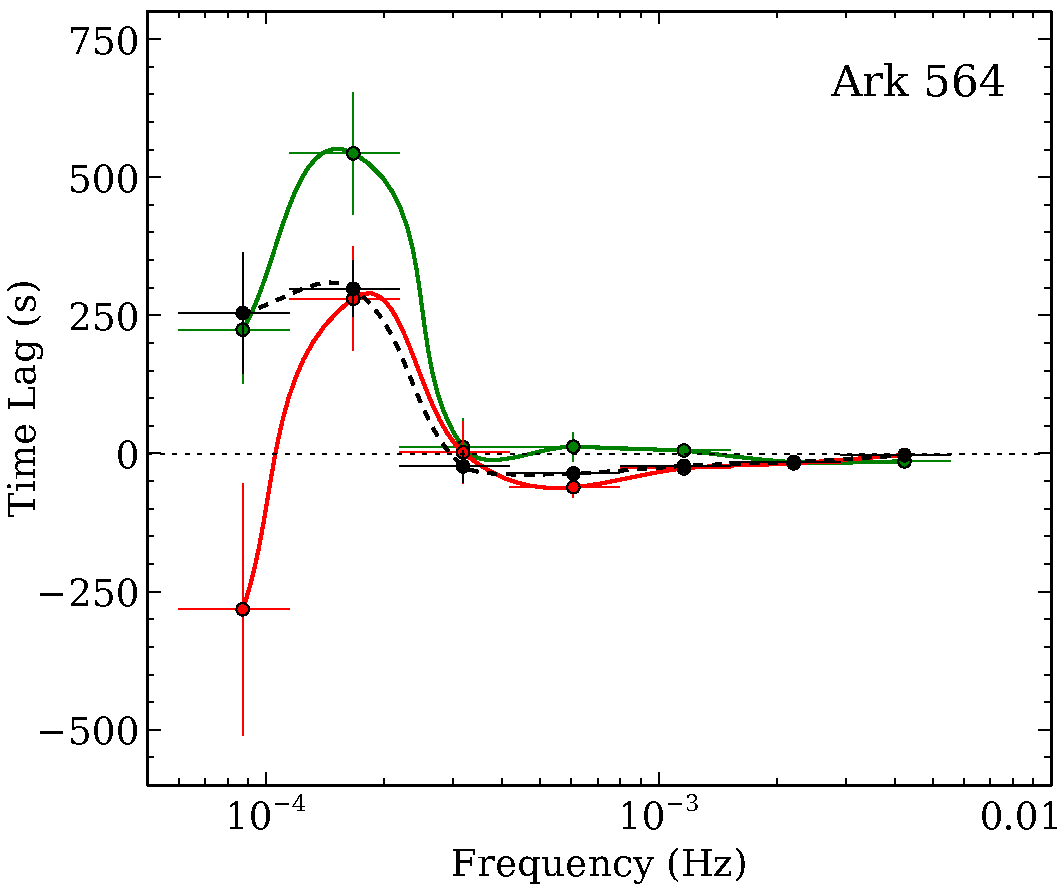
\includegraphics[scale=0.4]{images/Ark564-lag-results-lo-hi-flux-FP.pdf}
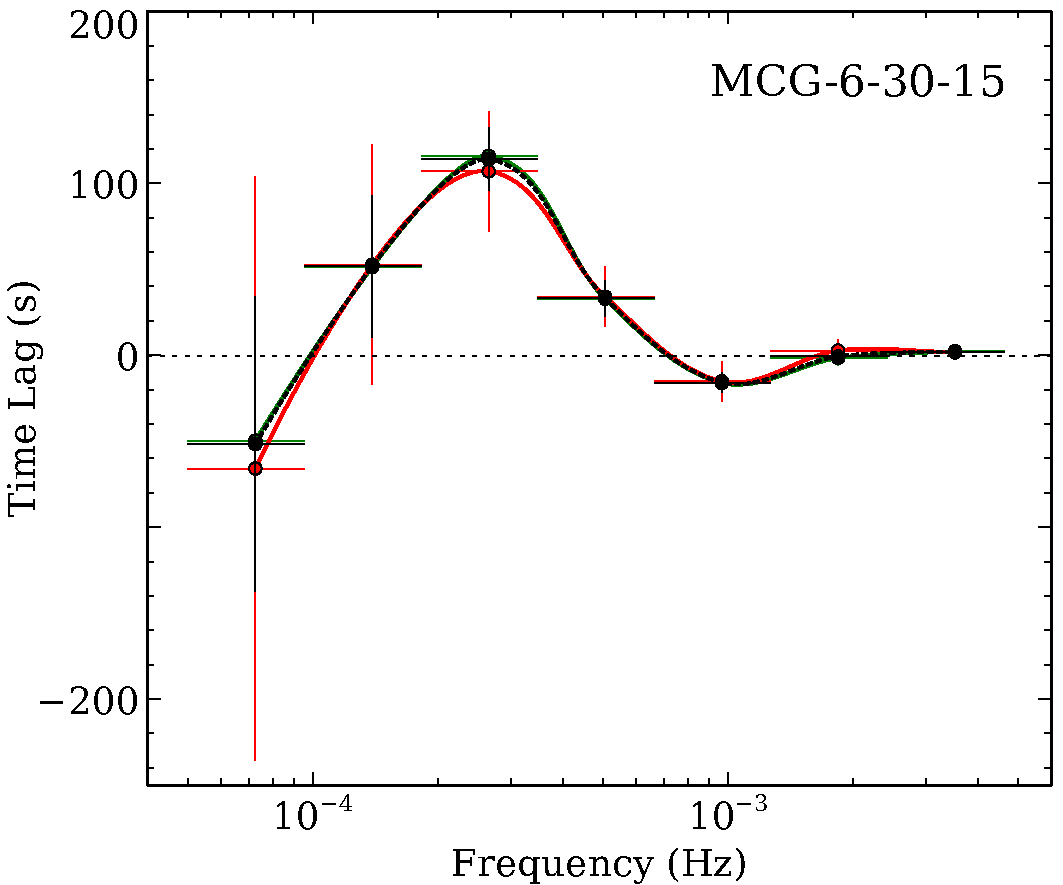
\includegraphics[scale=0.4]{images/MCG-lag-results-lo-hi-flux-FP.pdf}\\
\vspace{0.5cm}
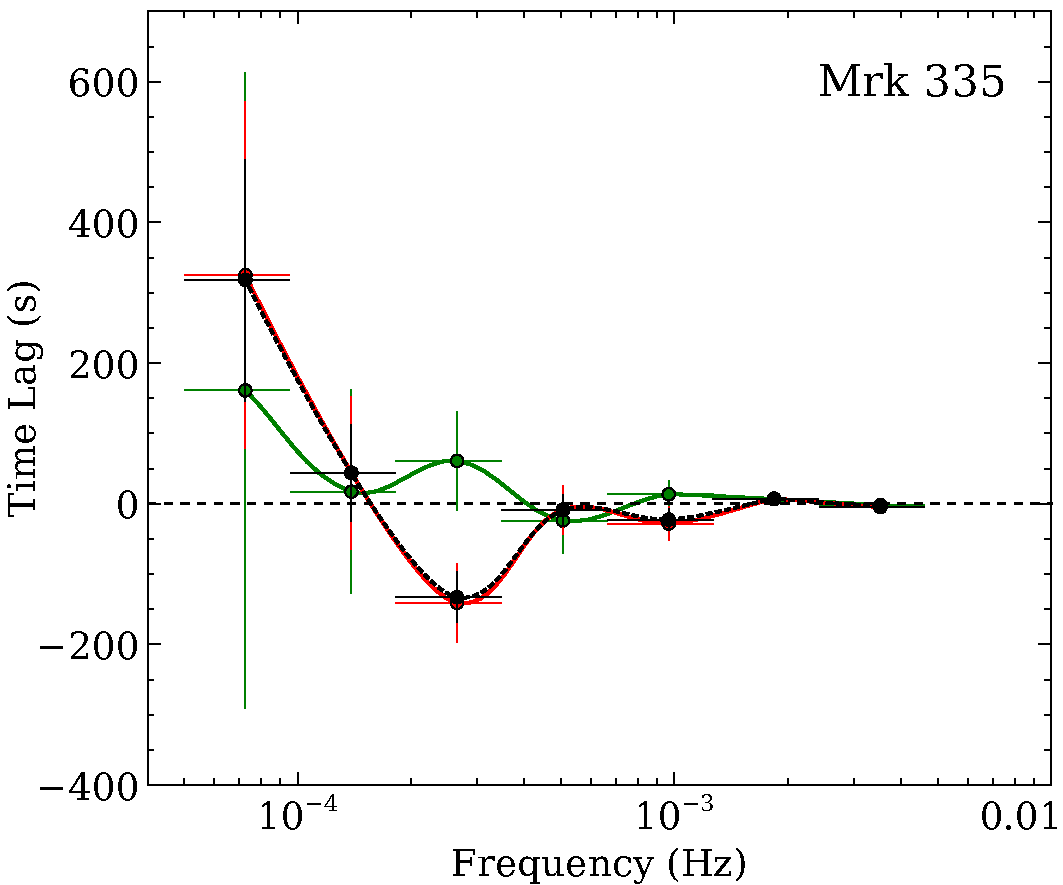
\includegraphics[scale=0.4]{images/Mrk335-lag-results-lo-hi-flux-FP.pdf}
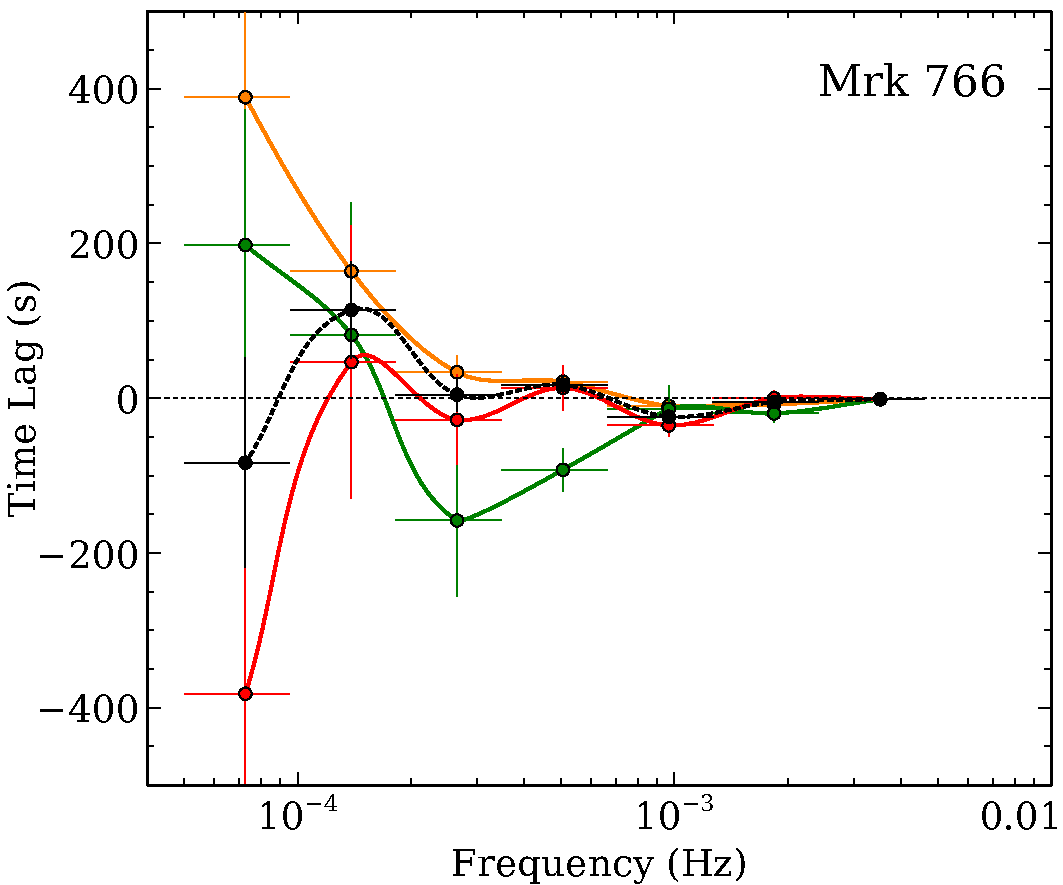
\includegraphics[scale=0.4]{images/Mrk766-lag-results-lo-hi-flux-FP.pdf}\\
\vspace{0.5cm}
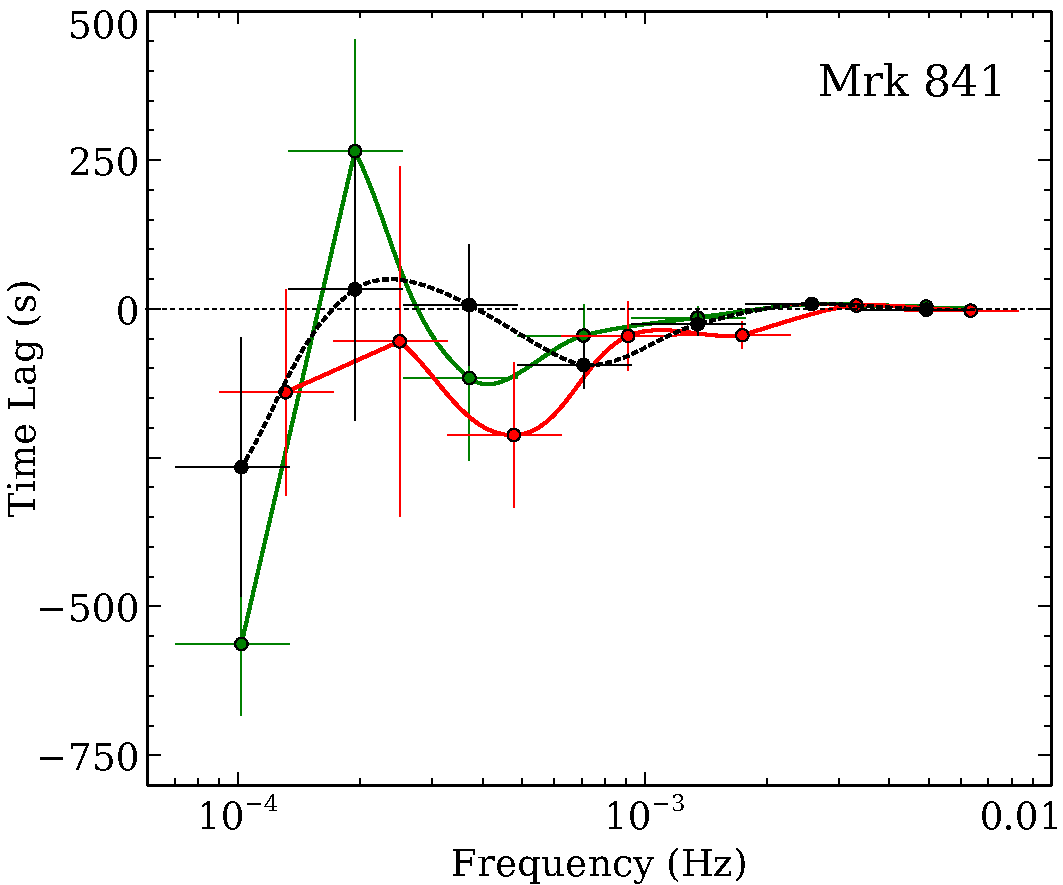
\includegraphics[scale=0.4]{images/Mrk841-lag-results-lo-hi-flux-FP.pdf}
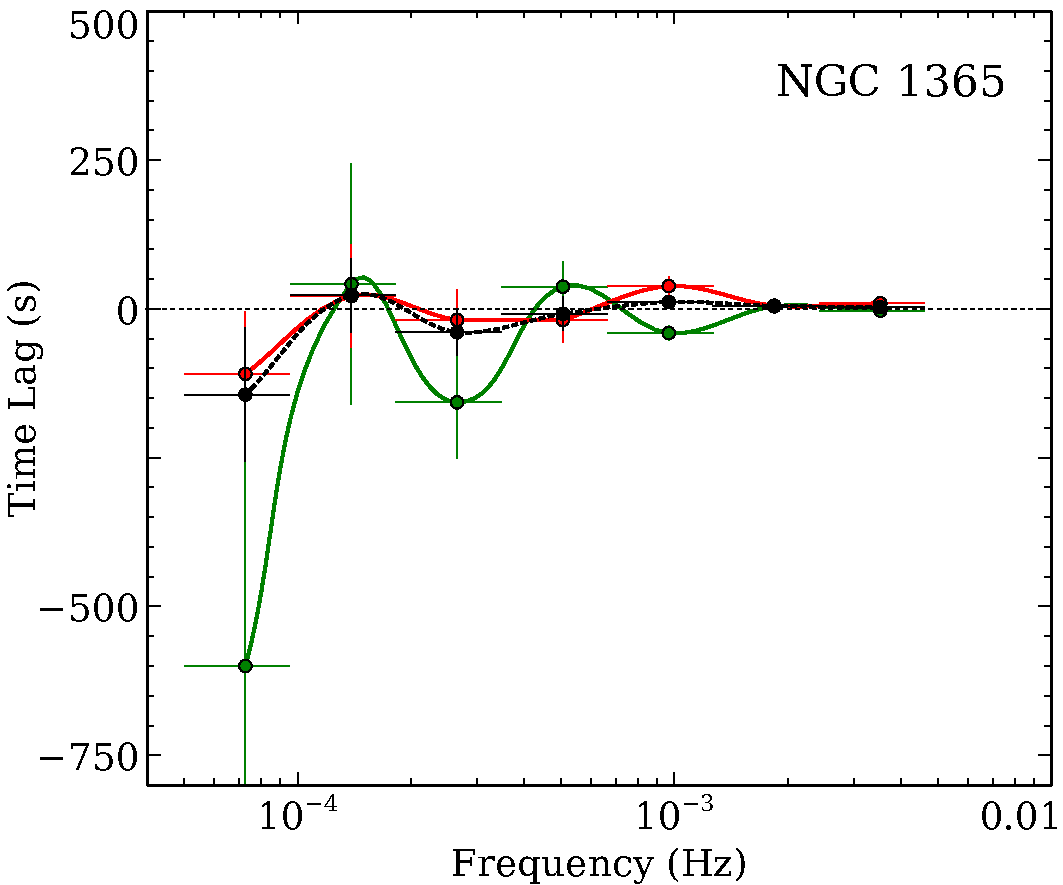
\includegraphics[scale=0.4]{images/NGC1365-lag-results-lo-hi-flux-FP.pdf}
\caption[The lag-frequency results]{The lag-frequency results for all other AGN in the sample list, showing the combined lags (black dashed lines), high flux (red), medium flux (amber) and low flux lags (green).  }
\label{fig:lagfreq-results}
\end{figure}
% /homeb/steff075/phd_ecm/MCG-6-30-15/lag-results-lo-hi-flux.vsz etc

\begin{figure}
    \ContinuedFloat
\centering
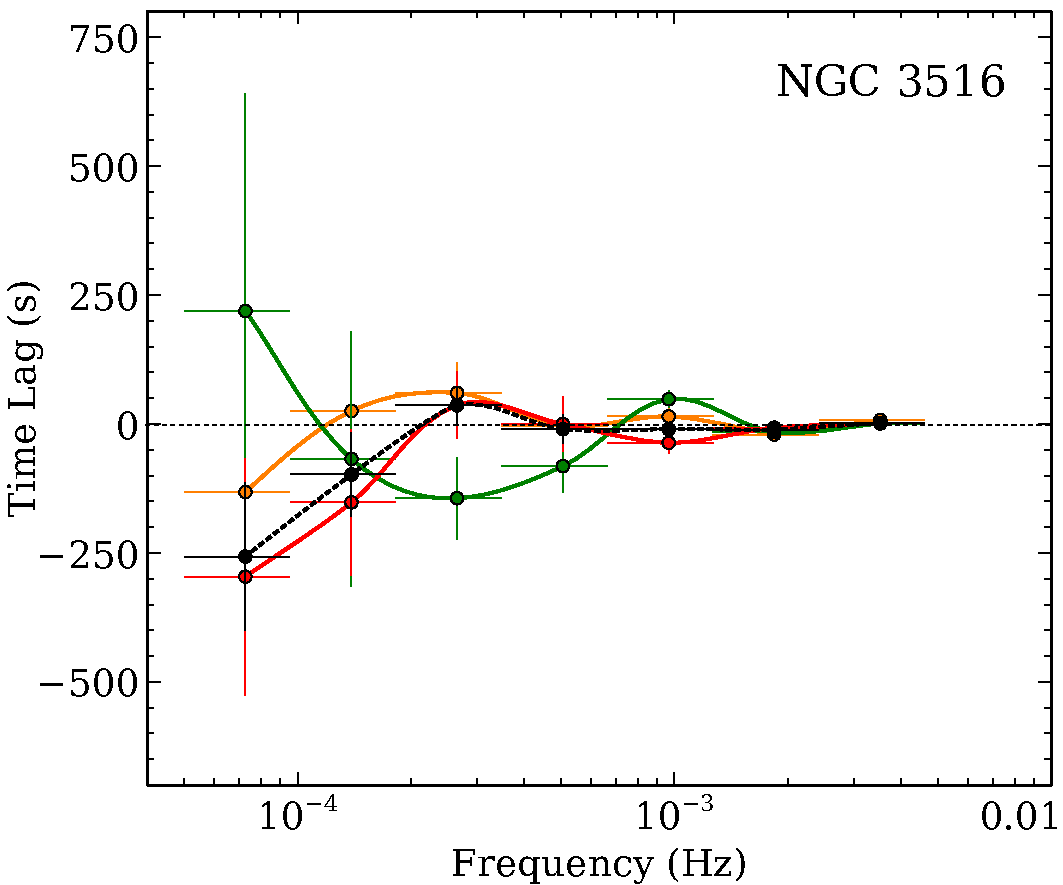
\includegraphics[scale=0.4]{images/NGC3516-lag-results-lo-hi-flux-FP.pdf}
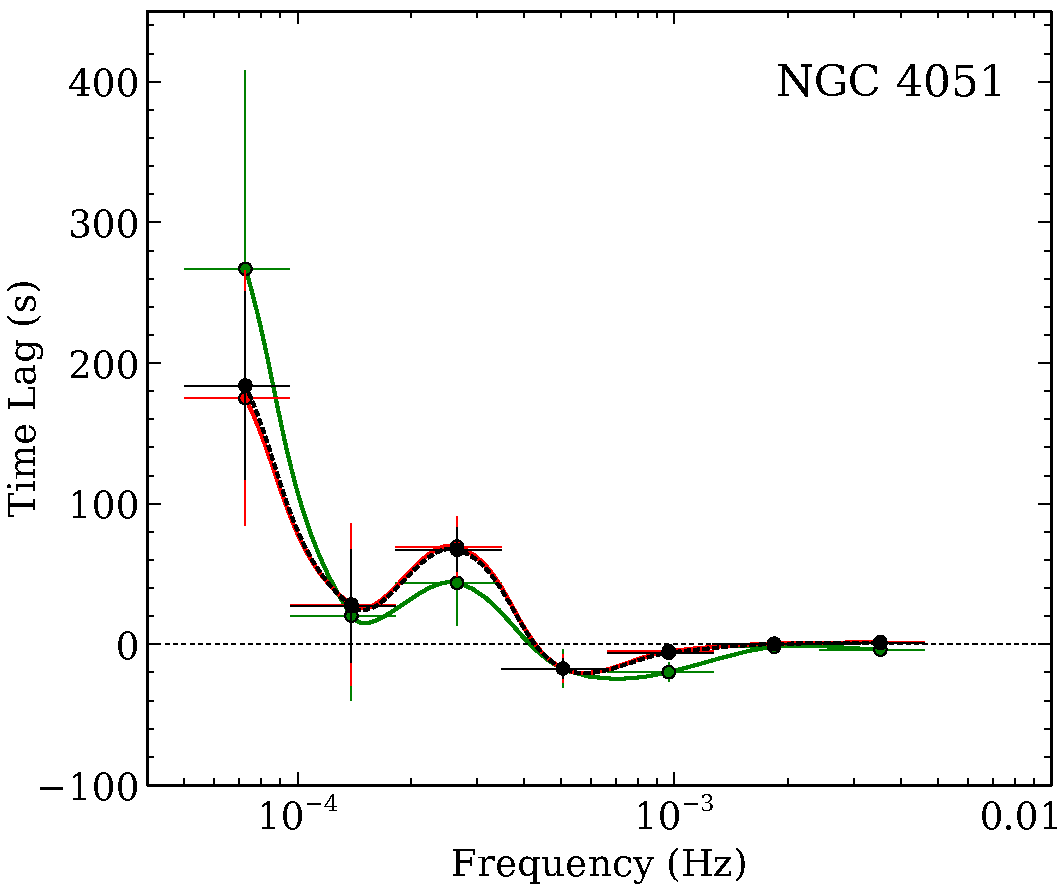
\includegraphics[scale=0.4]{images/NGC4051-lag-results-lo-hi-flux-FP.pdf}\\
\vspace{0.5cm}
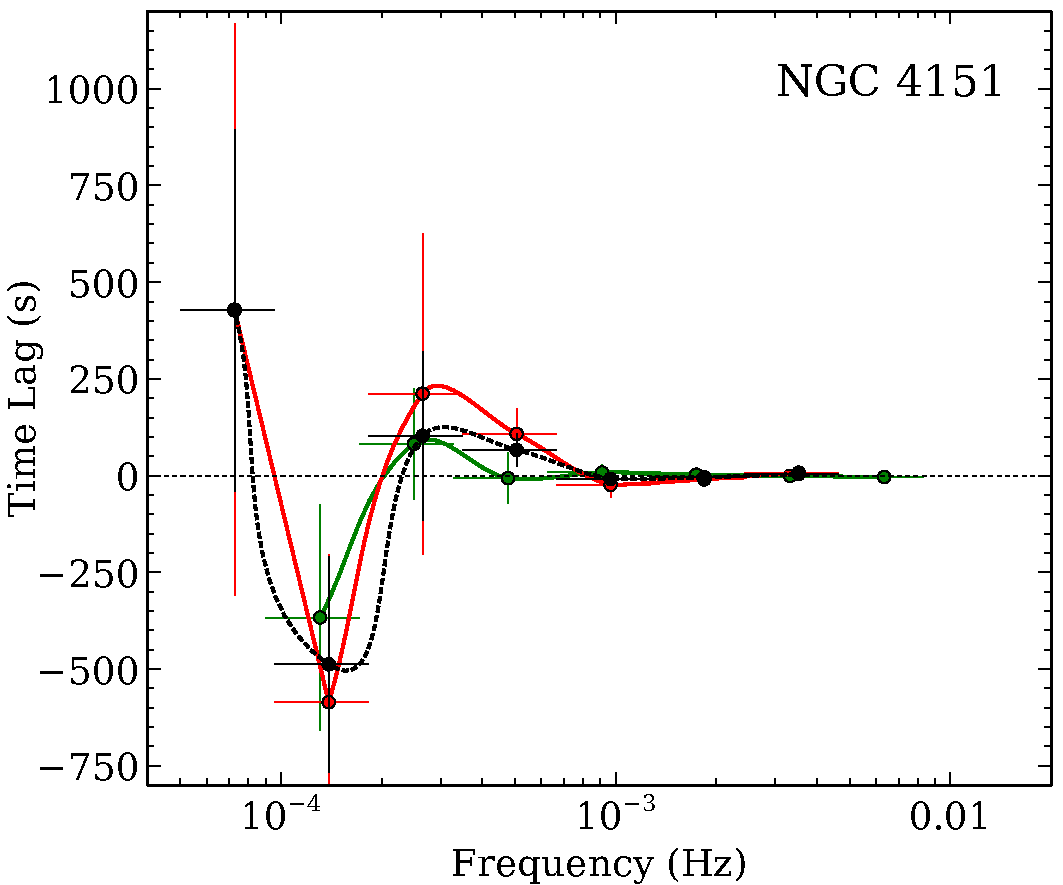
\includegraphics[scale=0.4]{images/NGC4151-lag-results-lo-hi-flux-FP.pdf}
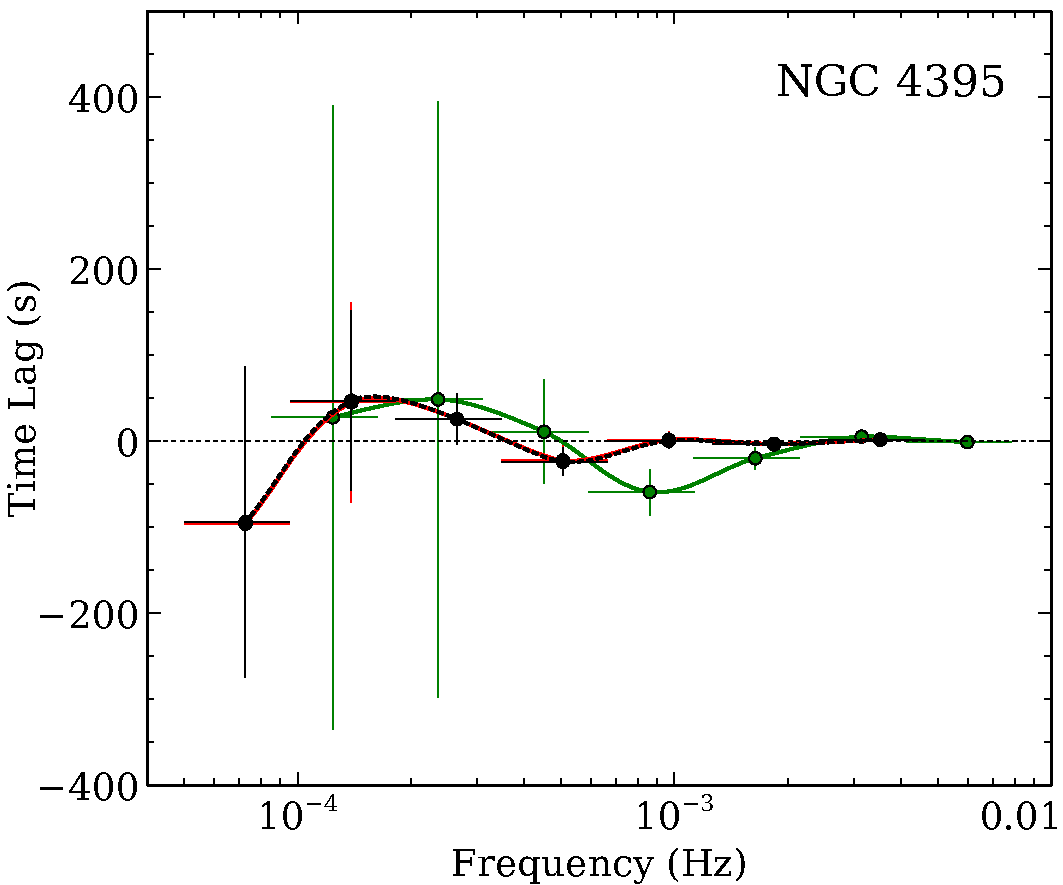
\includegraphics[scale=0.4]{images/NGC4395-lag-results-lo-hi-flux-FP.pdf}\\
\vspace{0.5cm}
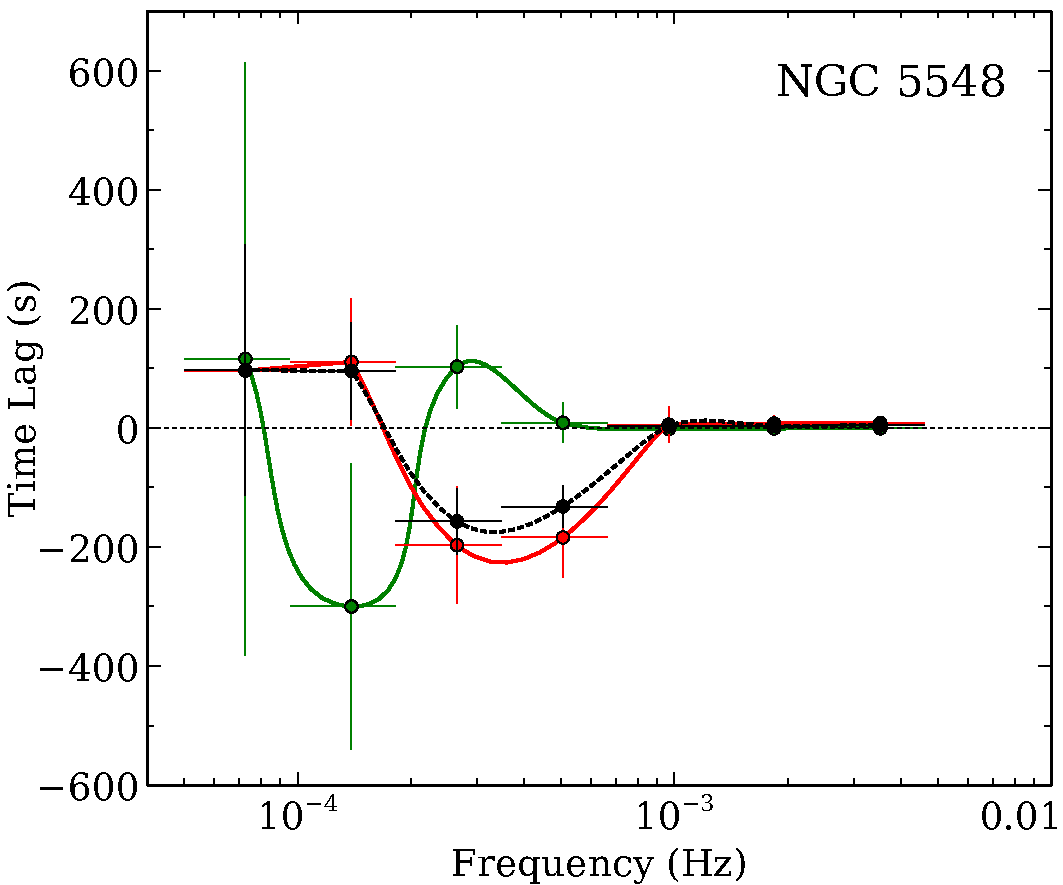
\includegraphics[scale=0.4]{images/NGC5548-lag-results-lo-hi-flux-FP.pdf}
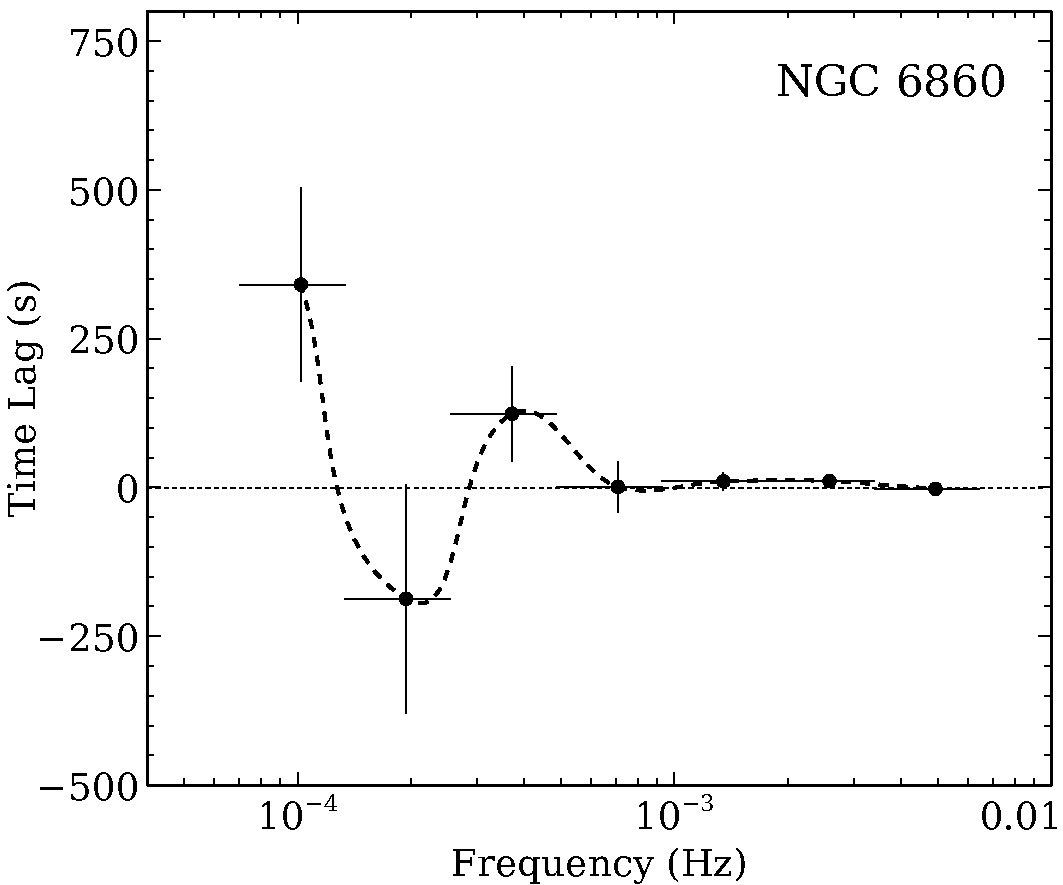
\includegraphics[scale=0.4]{images/NGC6860-lag-results-lo-hi-flux-FP.pdf}
\caption[The lag-frequency results (continued)]{The lag-frequency results (continued).}
%\label{fig:lagfreq-results}
\end{figure}

\begin{figure}
    \ContinuedFloat
\centering
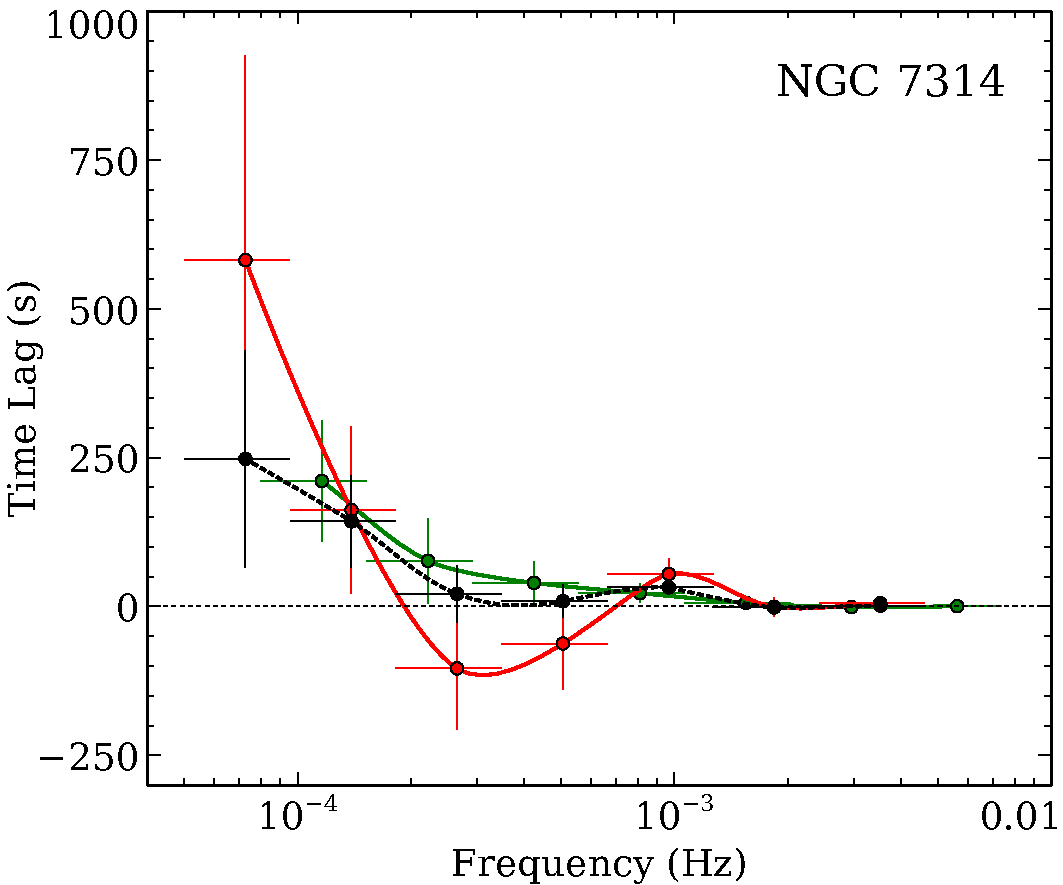
\includegraphics[scale=0.4]{images/NGC7314-lag-results-lo-hi-flux-FP.pdf}
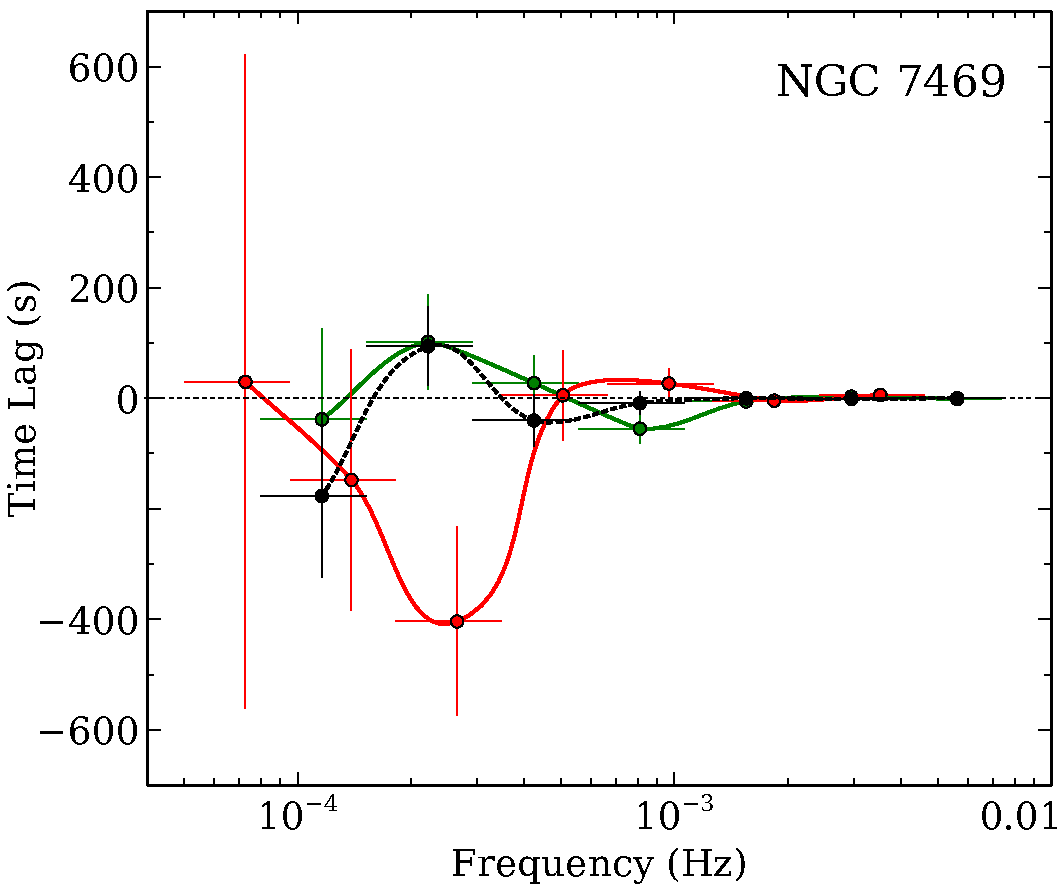
\includegraphics[scale=0.4]{images/NGC7469-lag-results-lo-hi-flux-FP.pdf}\\
\vspace{0.5cm}
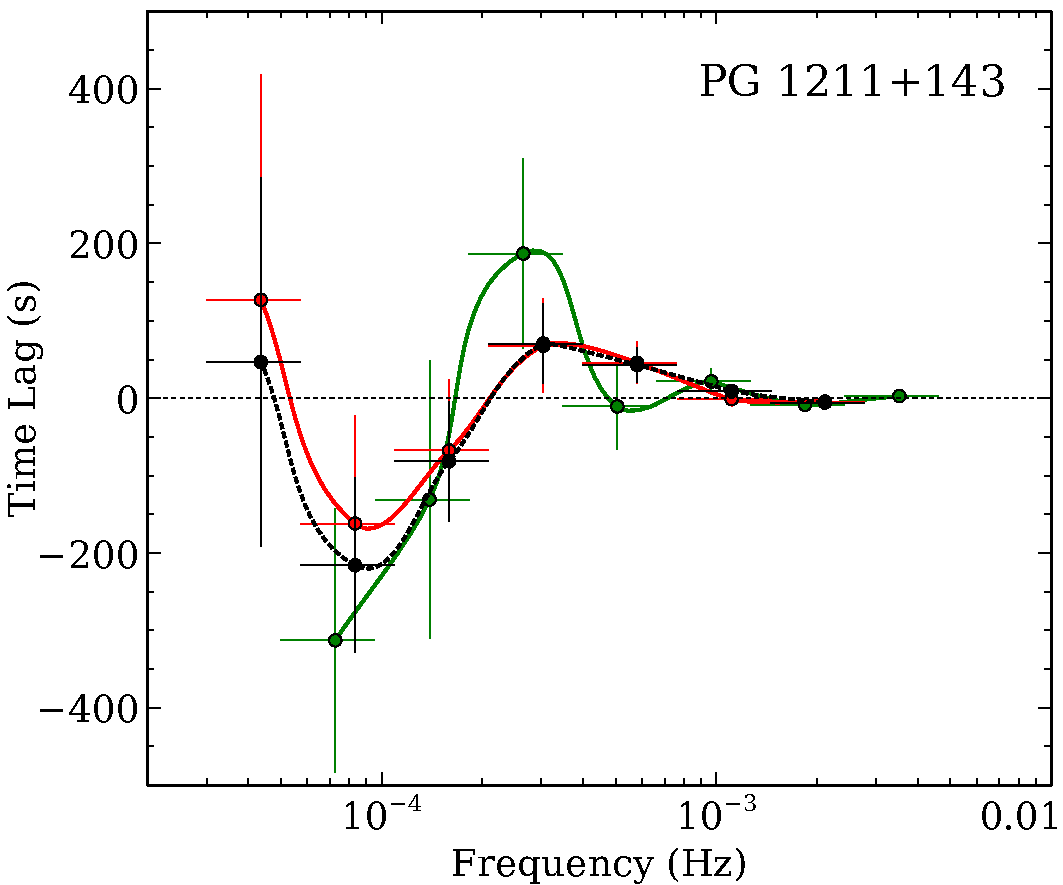
\includegraphics[scale=0.4]{images/PG1211+143-lag-results-lo-hi-flux-FP.pdf} 
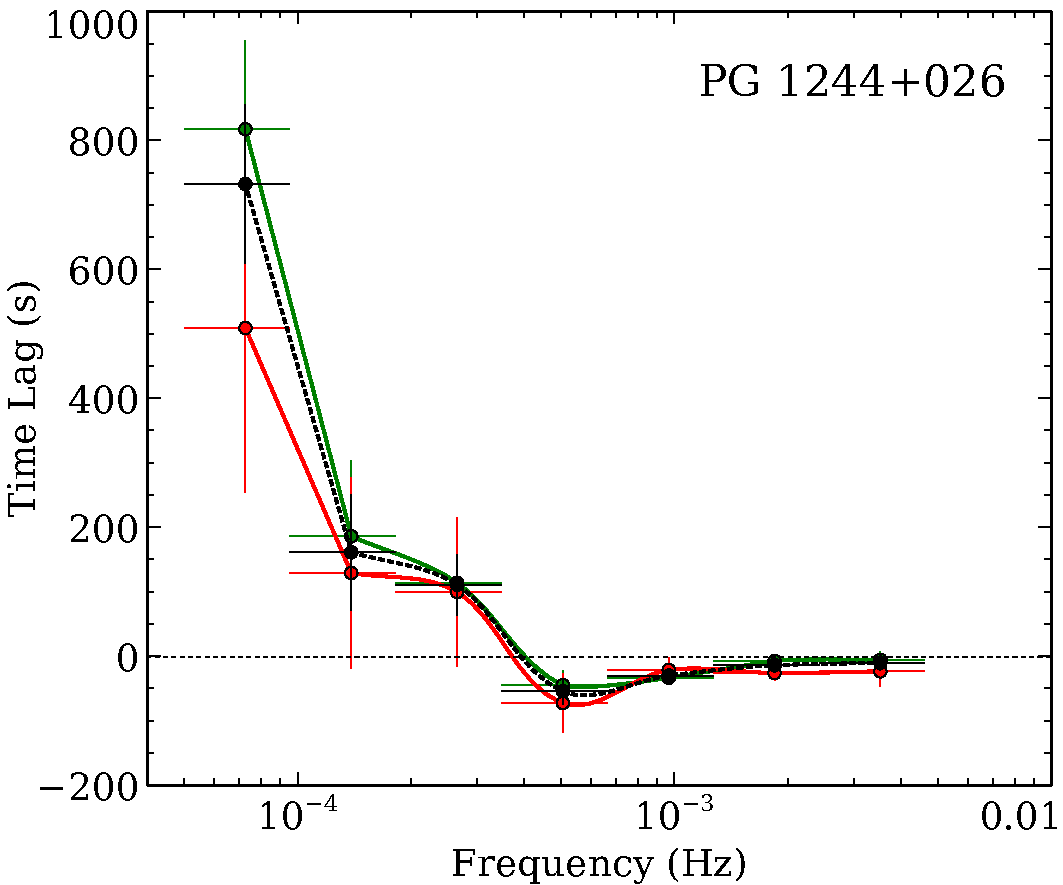
\includegraphics[scale=0.4]{images/PG1244+026-lag-results-lo-hi-flux-FP.pdf}\\
\vspace{0.5cm}
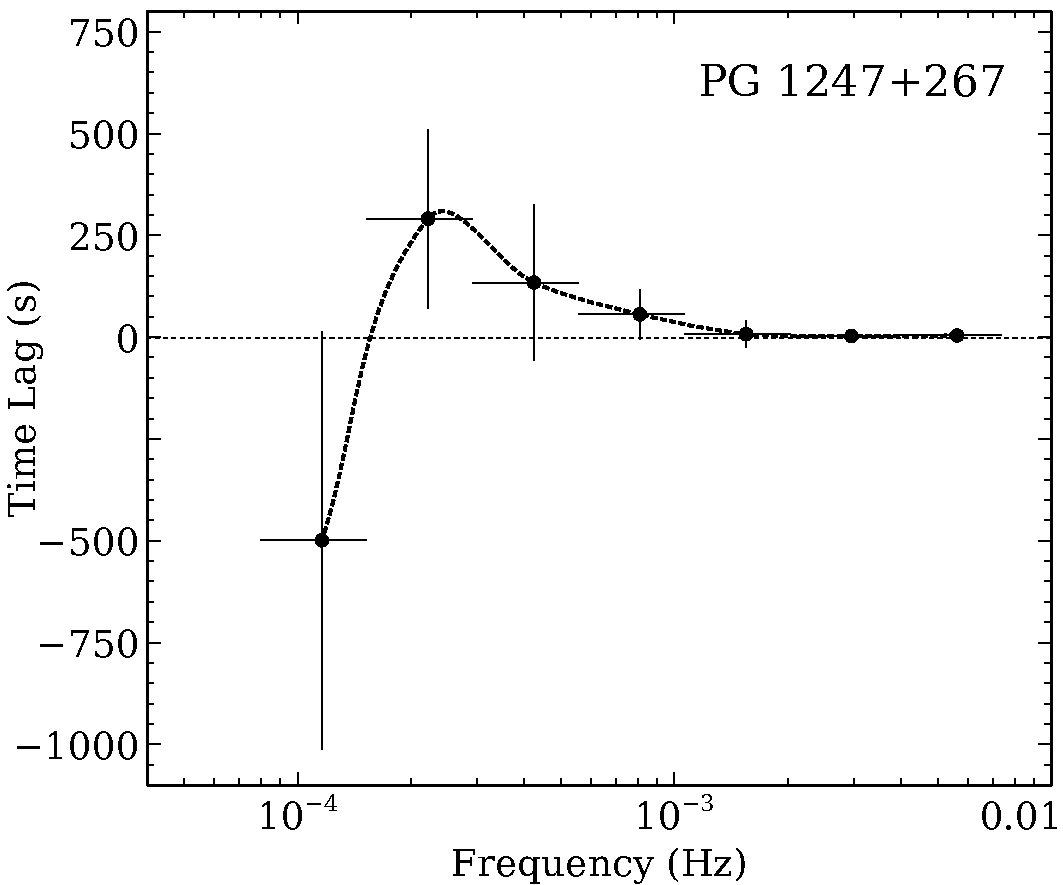
\includegraphics[scale=0.4]{images/PG1247+267-lag-results-lo-hi-flux-FP.pdf}
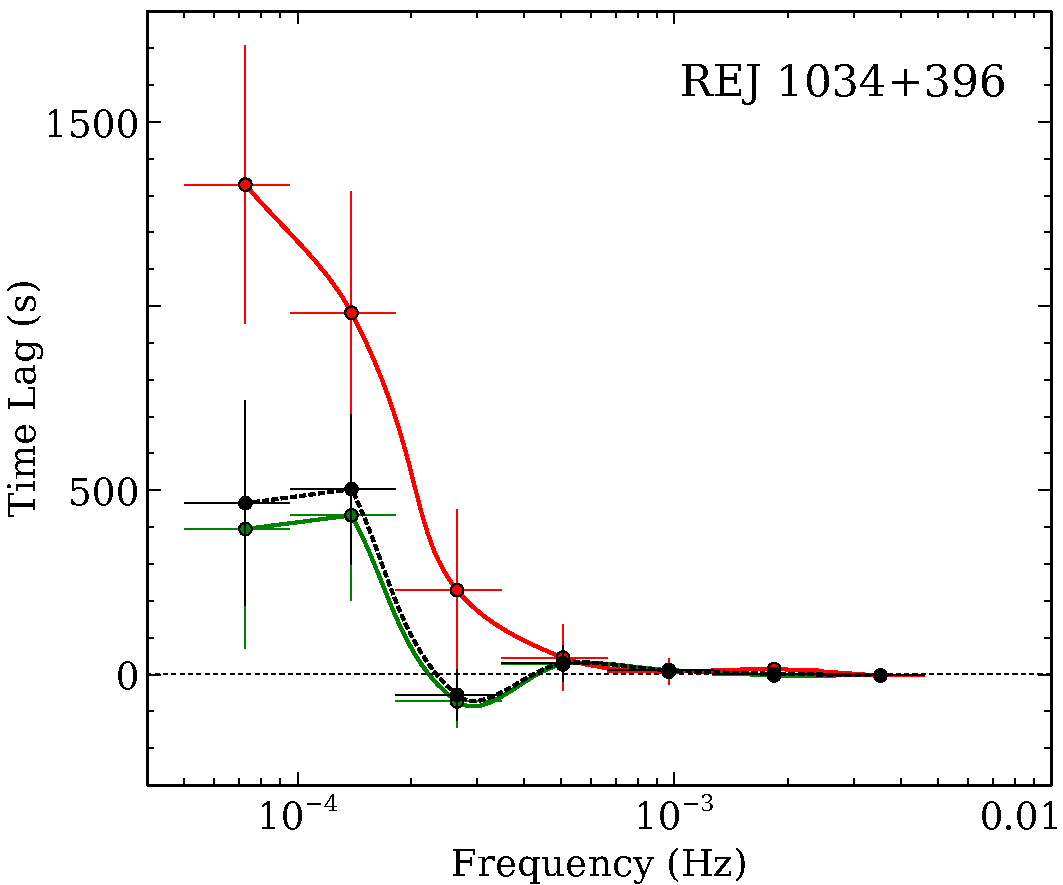
\includegraphics[scale=0.4]{images/REJ1034+396-lag-results-lo-hi-flux-FP.pdf}
\caption[The lag-frequency results (continued)]{The lag-frequency results (continued).}
%\label{fig:lagfreq-results}
\end{figure}





\end{landscape}
\end{document}
